\begin{center}
    \Large{\textbf{Практична частина}}
\end{center}

\vspace{1mm}

У результаті проведених експериментів 
були отримані наступні дослідні дані:

\begin{table}[h]
    \centering
    \begin{tabular}{|c|c|c|c|}
        \hline
        \textbf{Фільтр} & \textbf{Кільце} & \textbf{$r_{світ}$($5 \cdot 10^{-5}$м)} & \textbf{$r_{тем}$($5 \cdot 10^{-5}$м)} \\

        \hline
        \multirow{5}{*}{червоний} & 1 & 10 & 10,7 \\
        \cline{2-4}
        & 2 & 11.5 & 12.5 \\
        \cline{2-4}
        & 3 & 13.5 & 14 \\
        \cline{2-4}
        & 4 & 15 & 15.5 \\
        \cline{2-4}
        & 5 & 16 & 16.5 \\
        \hline
        
        \hline
        \multirow{5}{*}{помаранчевий} & 1 & 10 & 11 \\
        \cline{2-4}
        & 2 & 12 & 12.9  \\
        \cline{2-4}
        & 3 & 13.5 & 14.1 \\
        \cline{2-4}
        & 4 & 14.6 & 15  \\
        \cline{2-4}
        & 5 & 15.6 & 16  \\ 
        \hline

        \hline
        \multirow{5}{*}{зелений} & 1 & 9.3 & 10.3 \\
        \cline{2-4}
        & 2 & 11.2 & 11.7 \\
        \cline{2-4}
        & 3 & 12.5 & 13.1 \\
        \cline{2-4}
        & 4 & 13.6 & 14.1 \\
        \cline{2-4}
        & 5 & 14.4 & 15.0 \\
        \hline

        \hline
        \multirow{5}{*}{синій} & 1 & 9.9 & 10.8 \\
        \cline{2-4}        
        & 2 & 11.8 & 12.2 \\
        \cline{2-4}
        & 3 & 13.2 & 13.6 \\
        \cline{2-4}
        & 4 & 14.1 & 14.6 \\
        \cline{2-4}
        & 5 & 14.7 & 15.0 \\
        \hline

    \end{tabular}
    \caption{Дослідні дані}
\end{table}

З формул \ref{eq:4} і \ref{eq:5} бачимо, що значення радіуса 
кривизни $R$ та товщини зазору в місці контакту $d_0$ можна знайти 
розв'язав задачу лінійної регресіі, а саме, якщо $r^2 = k m + b$, то

$$ R = \frac{k}{\lambda} $$
$$ d_0 = - \frac{b_{тем}}{2R} = - \frac{b_{світ}}{2R} - \frac{\lambda}{4} $$

Діаметр плями, що утворилася між лінзою та скляною поверхней, з елементарних
геометричних міркувань(теорема Піфагора) можна образувати наступним чином:

$$ D = 2 \sqrt{R^2 - (R-d_0)^2} = 2 \sqrt{2R|d_0| - d_0^2} $$

Отже, обрахуємо $R$, як середнє значення результатів для світлих і темних 
кілець. Результати містяться у таблиці 3. Графіки отриманих залежностей наведені нижче(рис. 2, рис. 3).

\begin{table}[h]
    \centering
    \begin{tabular}{|c|c|c|c|c|c|c|c|c|c|c|c|c|}
        \hline
        \textbf{Фільтр} & \textbf{$R_{тем}$(см)} & \textbf{$R_{світ}$(см)} & \textbf{$R$(см)} &
        \textbf{$d_{0_{тем}}$(мкм)} & \textbf{$d_{0_{світ}}$(мкм)} & \textbf{$d_0$(мкм)} & \textbf{$D$(мкм)} \\
        \hline

        червоний & 14.147 & 14.33 & 14.24 & -0.67 & -0.68 & -0.68 & 877 \\
        \hline
        
        помаранчевий & 12.52 & 13.56 & 13.04 & -0.95 & -0.81 & -0.88 & 957 \\
        \hline
        
        зелений & 13.72 & 13.79 & 13.76 & -0.71 & -0.7 & -0.7 & 879 \\
        \hline

        синій & 16.19 & 17.04 & 16.61 & -0.72 & -0.67 & -0.7 & 962 \\
        \hline

    \end{tabular}
    \caption{Результати обчислень}
\end{table}



\begin{figure}[h!]    
    \centering
    \includegraphics[width=0.7\textwidth]{assets/r_dark(m).pdf}
    \caption{Графіки залежностей квадрату радіуса темних кілець від номера}
\end{figure}
\begin{figure}[h!]
    \centering
    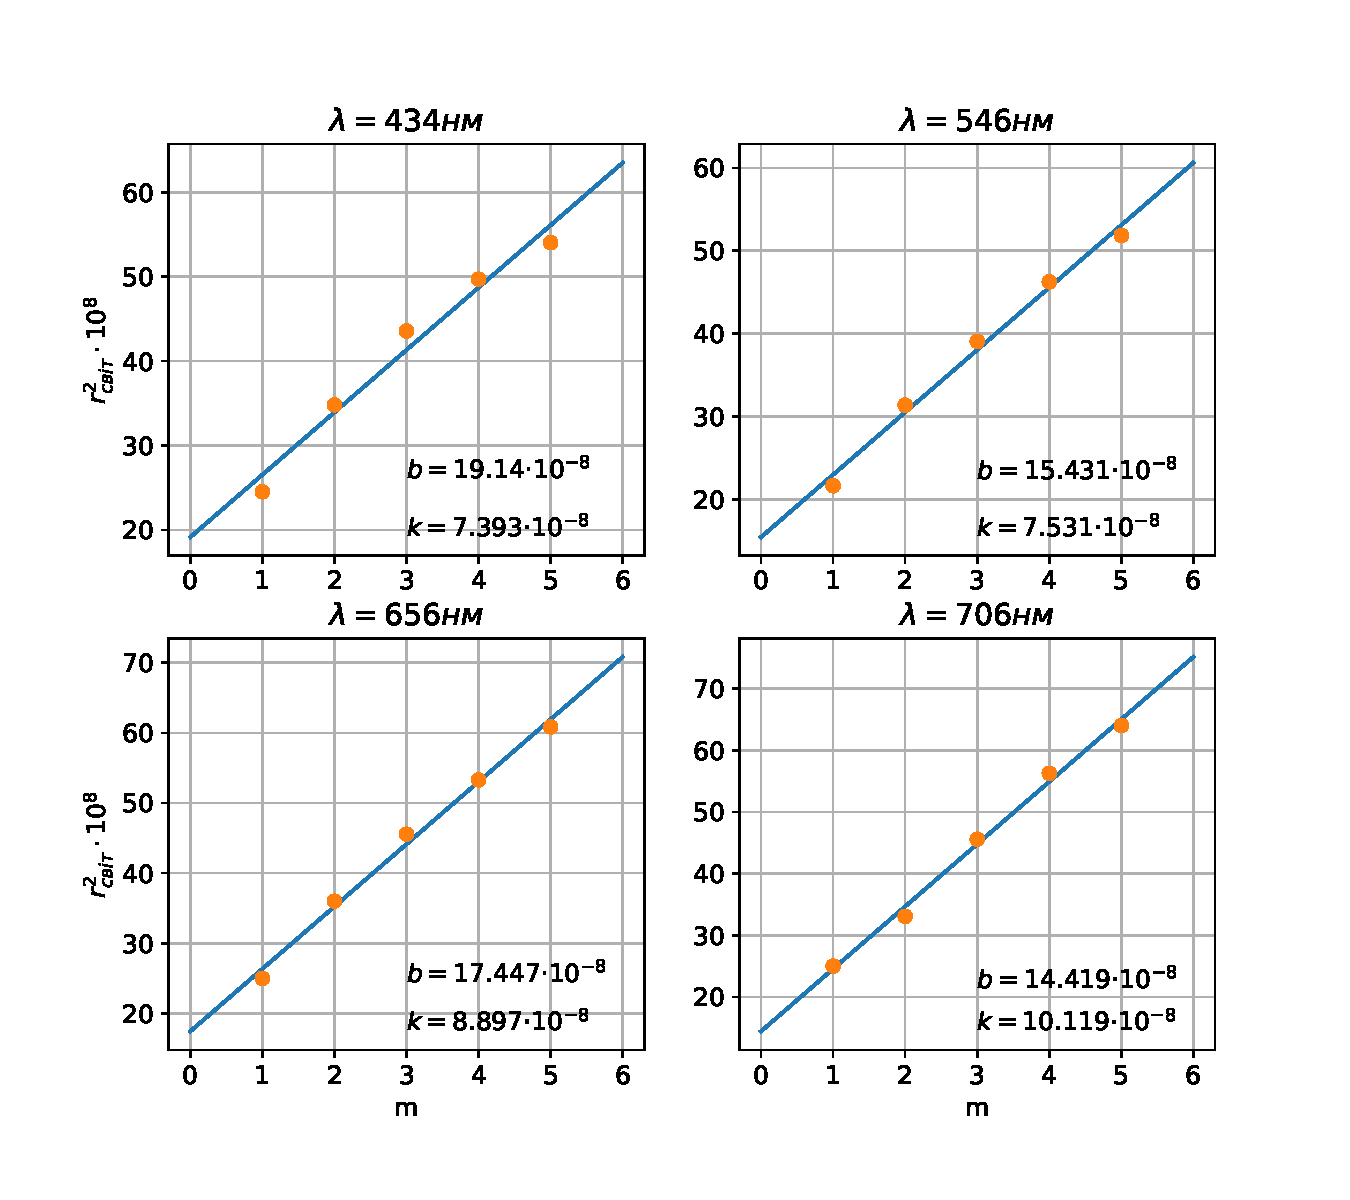
\includegraphics[width=0.7\textwidth]{assets/r_light(m).pdf}
    \caption{Графіки залежностей квадрату радіуса світлих кілець від номера}
\end{figure}

\pagebreak